\newcommand{\dstar}{\delta^{*}}
\section{Capa limite para placas planas}
Una placa plana inmersa en un fluido con velocidad relativa puede asemejarse a una lista variada de problemas de ingeniería desde aviones hasta intercambiadores de calor. El concepto de la capa límite es simplemente el interfaz virtual entre la zona donde dominan los efectos viscosos y la zona invíscida. 

Más precisamente:\textit{ La capa límite se dibuja como una linea donde la velocidad absoluta del flujo es 99\% de la velocidad del flujo ``en el infinito"{}}($U_\infty$).\footnote{Sobre la capa límite y toda la región inviscida se desprecia $\spartial{u}{y}$, el cual es proporcional al corte $\tau$.}

 Para el estudio de capas limites se parte de las hipótesis 
 
 \begin{itemize}
 	\item Flujo bidimensional $u_j = u \hat{\i} + v \hat{\j}$
 	\item Estacionario
 	\item Incompresible $ \spartial{u}{x}+\spartial{v}{y}=0$
 	\item Newtoniano  $\tau_{xy}=\mu \spartial{u}{y}$
 	\item Isotérmico $\spartial{T}{x}=\spartial{T}{y}=0$
 \end{itemize}

 Cantidad de movimiento:
\[
\rho\left(u\spartial{u}{x}+v\spartial{u}{y}\right)=\mu \dpartial{u}{y}-\spartial{p}{x}
\]

Solo se van a estudiar capas límites para Números de Reynolds altos $\Reynolds_\delta\gg 1$.\footnote{Un número adimensionales con un subíndice indica que longitud característica tomar. Por ejemplo: $\Reynolds_D= \frac{UD}{\nu}$}

\begin{figure}%[tb]
    \centering
    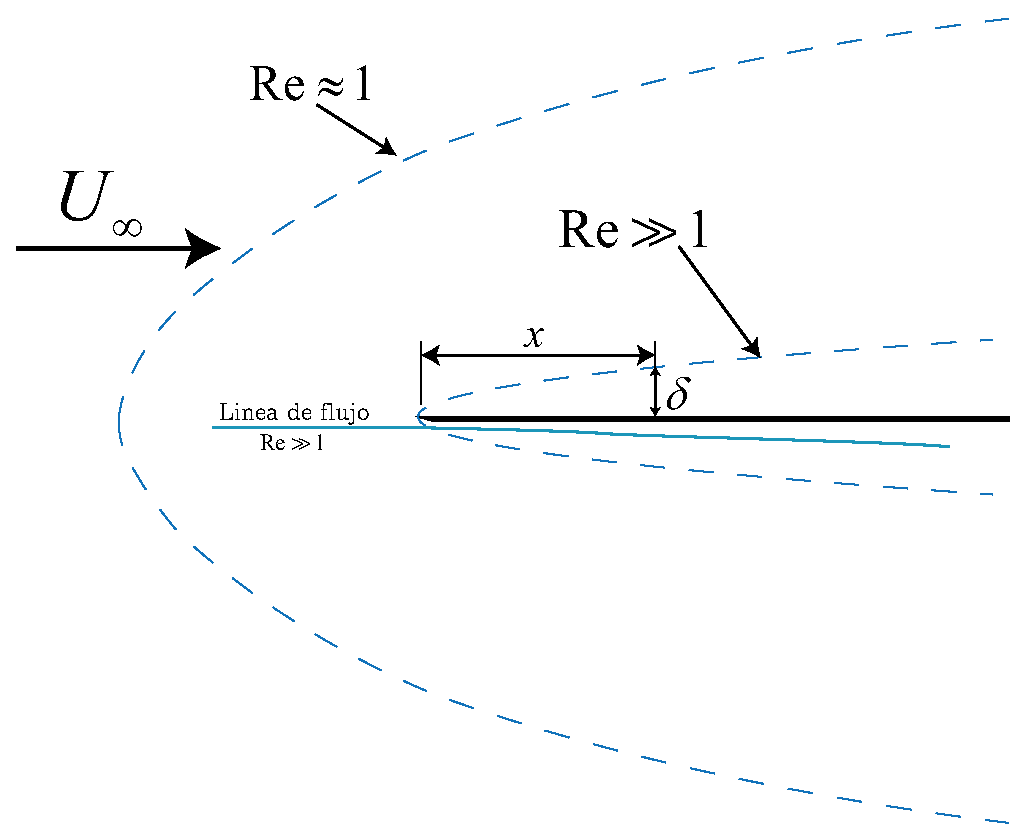
\includegraphics[width=0.47\textwidth]{fig/BL1.eps}
    \caption{Dos casos de capa límite muy diferente. Se va tratar capas límites con $\Reynolds_\delta \gg1$.}
    \label{fig:BLintro}
\end{figure}
\subsection{Solución analítica: Laminar}\label{ssec:capalimLaminar}
En 1908 Paul Richard Heinrich Blasius, un físico alemán, desarrolla la teoría fundamental para el estudio de capa limites laminares sobre placas planas. Mediante un uso riguroso de la teoría de semejanza llega a la siguiente ecuación diferencial
\[
ff^{\prime\prime}+2f^{\prime\prime\prime}=0
\]
cuya solución (obtenida numéricamente con determinadas condiciones de borde) se denomina el perfil de velocidades de Blasius.
\[
\begin{array}{lll}
u(x,0)=0, & u(x,\delta)=U_\infty, & \tau|_{y=\delta} =0
\end{array}
\]

En base a este perfil de velocidades se desarrollan las siguientes relaciones \citep{durst2008fluid}:
\begin{equation}
    \delta=\frac{5,2x}{\sqrt{\Reynolds_x}}=5,2\sqrt{\frac{x\mu}{\rho U_\infty}}
\end{equation}

\begin{equation}
    \tau_s=\mu \left. \spartial{u}{y}\right|_{y=0}=0,332\,\mu\frac{U_\infty}{x}\sqrt{\Reynolds_x}=0,332\, U_\infty^{1,5}\sqrt{\frac{\rho}{x\mu}}
\end{equation}
donde $\tau_s$ es el la tensión de corte sobre la superficie de la placa. 

\begin{equation}
    c_f=\frac{\tau_s}{\rho U_\infty^2/2}=\frac{0,664}{\sqrt{\Reynolds_x}}
\end{equation}

\begin{equation}
    C_D=\bar{c}_f=\frac{1}{L}\int_0^Lc_f\di x=\frac{1,328}{\sqrt{\Reynolds_L}}
\end{equation}
donde $c_f$ es el coeficiente de fricción local sobre la placa y $C_D$ es el coeficiente de drag de la placa. La fuerza sobre la placa entera se puede entonces obtener dimensionalizando $C_D$ tal que
\[
F_D=\tfrac{1}{2}C_D \rho U_\infty A
\]

Las relaciones anteriores solo valen para régimen laminar. Se puede suponer que cualquier flujo $\Reynolds_L<\Reynolds_{\crit}=\num{5e5}$ es laminar. Si el flujo no es perturbado y la superficie de la placa es pulida se puede demorar la transición a turbulento hasta $\Reynolds_{\crit}=\num{3e6}$ \citep{kreith2011principles}.

\subsubsection*{Efecto desviador de lineas de flujo}
A causa de la desaceleración del flujo cerca de la placa las lineas de flujo se tiene que desviar hacia afuera. 

Para el caso de la figura \ref{fig:displthickness} se tiene una placa plana con flujo $U_\infty$ incidente. En color (linea solida) esta dibujado la capa límite. Para hallar $\dstar$ se plantea un VC que siga la linea de flujo del punto $(x,y)=(0,h)$ hasta $(x,y)=(x_0,\delta)$. La incógnita es $h$ y se puede hallar planteando conservación de masa entre la entrada y salida del VC.

\begin{equation}
    \dstar \approx \frac{\delta}{3}  \qquad \textrm{donde}\qquad  \delta=h+\dstar
\end{equation}


\begin{figure}[htb!]
    \centering
    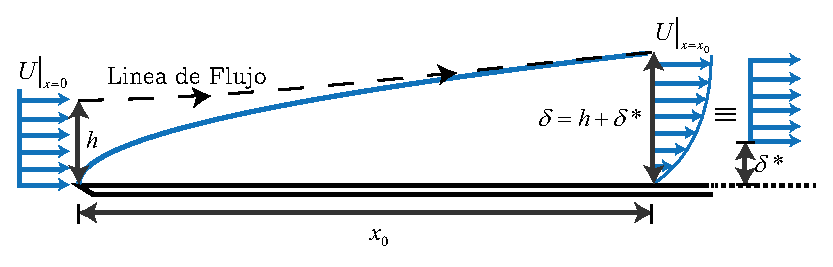
\includegraphics[width=0.47\textwidth]{fig/BLdispthick.eps}
    \caption{Efecto desviador de lineas de flujo y su efecto ``simulado"{} visto a la derecha.}
    \label{fig:displthickness}
\end{figure}

Demostración partiendo de conservación de caudal entre la entrada y salida donde $b$ es el ancho de la placa

\begin{gather*}
	\rho b \int^h_0 u(0;y)\di y = \rho b \int^{h+\dstar}_0 \!\!\!\!u(L;y)\di y \\
	\cancel{\rho b} h U_\infty =\cancel{\rho b}\int^{h+\dstar=\delta(x)}_0 \!\!\!\!\!\!\left[u(x;y)+U_\infty-U_\infty \right]\di y\\	
	\cancel{hU_\infty} = \int^{\delta(x)}_0 \!\!\!\!\!\!\left[u(x;y)-U_\infty \right]\di y+U_\infty (\cancel{h}+\dstar)
\end{gather*}
\begin{equation}
	\dstar = \int_0^{\delta(x)} \!\!\!\left(1-\frac{u(x;y)}{U_\infty} \right) \di y
\end{equation}


%%%%%%%%%%%%%%%%%%%%%%
%% TURBULENTO
%%%%%%%%%%%%%%%%%%%%%%

\subsection{Relación empírica: Turbulento}
En realidad una capa límite laminar siempre precede la turbulenta. Sin embargo el comienzo turbulencia se puede inducir sobre el filo de la placa usando alambre. Esto suele ser útil para aumentar la transferencia de calor y reducir el arrastre alto en régimen laminar.

Para flujo turbulento el espesor de capa límite no tiene solución exacta. Una relación empírica que se puede usar es la siguiente:
\begin{equation}
    \delta \approx \frac{0,22x}{\Reynolds_x^{\frac{1}{6}}}
\end{equation}

Prandtl sugiere usar (resultado final simplificado):
\[
c_f \approx 0,02\, \Reynolds_\delta^{-\frac{1}{6}} = 0,02\left(0,22 \Reynolds_x^{5/6}\right)^{-\frac{1}{6}}\approx \frac{0,026}{\Reynolds_x^{\frac{1}{7}}} 
\]

Otra formula que se puede usar \citep{kreith2011principles}:
\begin{equation}
    c_f=\frac{0,0576}{\Reynolds_x^{0,2}}
\end{equation}
No se pueden calcular los esfuerzos viscosos en la pared debido a la singularidad en $y=0$.

\[
\frac{\left\langle u \right\rangle}{U_\infty} = \left(\frac{y}{\delta} \right)^{\frac{1}{n}}, \quad n=7,8,9
\]
\subsubsection{Análisis capa mixta}

En el caso que demore la transisción a régimen turbulento se puede obtener la capa límite al final de la placa $\delta_L=\delta_{\mathrm{turb}}(L-x_0)$ despejando $x_0$ en
\[
\delta_\crit =\delta_{\mathrm{lam.}}(x_\crit) = \delta_{\mathrm{turb.}}(x_\crit-x_0) 
\]
donde $\Reynolds(x_\crit) =\Reynolds_{\crit}$, según lo visto en la sección \ref{ssec:capalimLaminar}.

\begin{figure}[htb!]
	\centering
	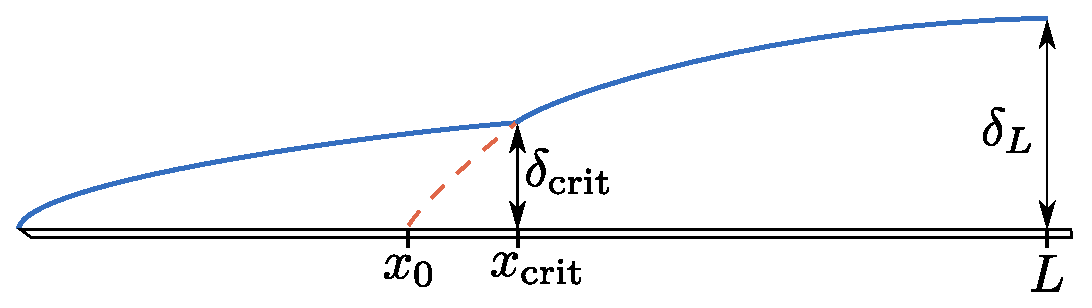
\includegraphics[width=0.48\textwidth]{fig/BLmixed.eps}
	\caption{Análisis de capa límite mixta.}
	\label{fig:BLmixed}
\end{figure}



\begin{figure}[htb!]
    \centering
    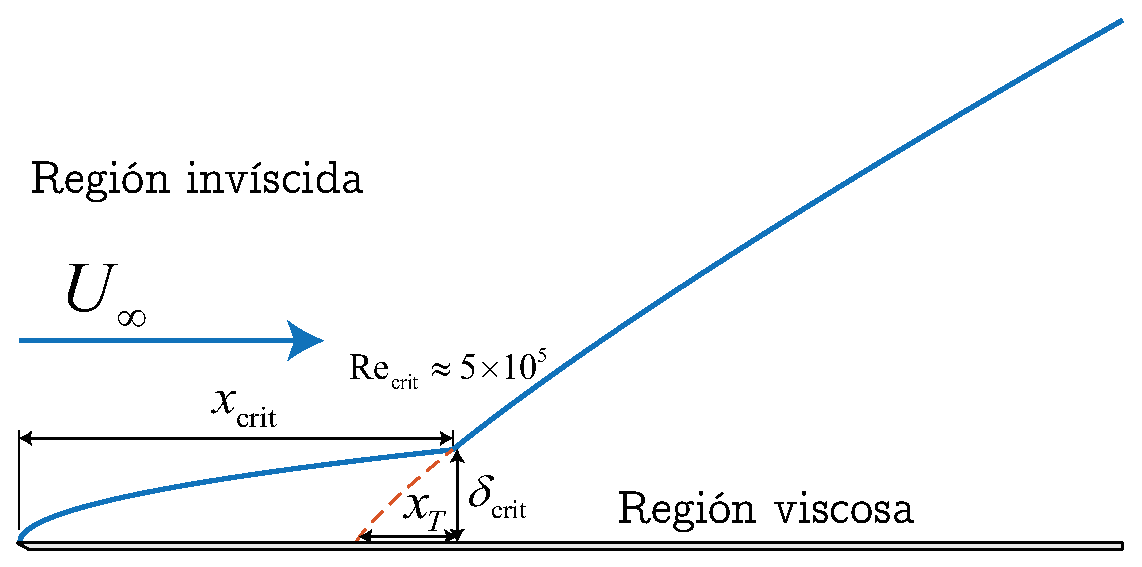
\includegraphics[width=0.48\textwidth]{fig/BLmixedejemplo.eps}
    \caption{Análisis de capa límite mixta de aire sobre una placa $L=10\si{\meter}$, $U_\infty=2\si{\meter\per\second}$. Resuelto en \Matlab.}
    \label{fig:BLmixedExample}
\end{figure}

\section{Flujo Potencial}
\subsection{Flujo potencial generalizado para 3-D}
La teoría de flujo potencial es útil para tratar problemas aerodinámicos e hidrodinámicos cuando se tiene un flujo invíscido (zona afuera de la capa límite) por su bajo costo computacional.

Hipótesis flujo potencial
\begin{itemize}
    \item Flujo invíscido
    \item Flujo irrotacional
    \item Régimen estacionario
\end{itemize}
Entonces existe una función potencial $\varphi$ tal que
\[
u_j = \partial_j \varphi \qquad \nabla^2\varphi = 0
\]
la segunda ecuación es equivalente a decir que el flujo es incompresible. La ecuación de Euler \eqref{eq:eulerDiff} es valida y se puede usar un Bernoulli de la forma
\begin{equation}
    \spartial{\varphi}{t}+\frac{p}{\rho}+\frac{||\partial_j \varphi||^2}{2}+gh=\textrm{const.}
\end{equation}
donde $h$ es la altura en el punto en cuestión, sea medido en $x,y$ o $z$.
\subsection{Flujo Potencial 2-D}

